\documentclass[a4paper,14pt]{extarticle}

\usepackage[left=30mm, right=10mm, top=20mm, bottom=20mm]{geometry}

\usepackage{amssymb}
\usepackage{amsmath}
\usepackage{tikz}
\usepackage{pgfplots}

\usepackage{graphicx}
\usepackage{setspace}

\usepackage{minted}
\usepackage{xcolor}

\usepackage{siunitx}
\usepackage{booktabs}
\usepackage{multirow}

\usepackage[T2A]{fontenc}
\usepackage[utf8]{inputenc}
\usepackage[russian]{babel}
\usepackage{tempora}
\usepackage{type1cm}
\usepackage{indentfirst}

\usepackage{caption}
\usepackage{subcaption}
\usepackage[hidelinks]{hyperref}
\usepackage[russian]{cleveref}
\usepackage{bookmark}

\pgfplotsset{compat=1.18}

\onehalfspacing

\renewcommand{\theFancyVerbLine}{%
	\sffamily\small\color{black}\arabic{FancyVerbLine}%
}

\definecolor{codebg}{rgb}{0.12,0.12,0.14}
\definecolor{codeframe}{rgb}{0.40,0.40,0.45}
\definecolor{keywordcolor}{rgb}{0.45,0.65,1.0}
\definecolor{stringcolor}{rgb}{1.0,0.55,0.45}
\definecolor{commentcolor}{rgb}{0.55,0.75,0.60}
\definecolor{textcolor}{rgb}{0.90,0.90,0.90}

\setminted{
    bgcolor=codebg,
	fillcolor=codebg,
	framesep=1em,
	frame=single,
    rulecolor=\color{codeframe},
    fontsize=\normalsize,
    baselinestretch=1.1,
    linenos,
    numbersep=6pt,
    tabsize=4,
    breaklines,
    breakbytoken,
	breaksymbolleft={},
    autogobble,
    showspaces=false,
    showtabs=false,
}

\usemintedstyle{lightbulb}
\setmintedinline{
    bgcolor=codebg
}

\makeatletter
\setlength{\@fptop}{0pt}
\setlength{\@fpsep}{8pt}
\setlength{\@fpbot}{0pt plus 1fil}
\makeatother

\newcommand{\circledequals}{\mathbin{\tikz \node[draw,circle,inner sep=1pt] {$=$};}}

\DeclareMathOperator{\Bernoulli}{Bernoulli}

\begin{document}
    \begin{titlepage}
		\centering
		
		
\includegraphics{images/FEFU-logo.jpg}\\
		МИНИСТЕРСТВО ОБРАЗОВАНИЯ И НАУКИ РОССИЙСКОЙ ФЕДЕРАЦИИ\\
		Федеральное государственное автономное образовательное учреждение высшего образования\\
		\textbf{«Дальневосточный федеральный университет»}

		\rule{\linewidth}{0.8mm}\\[0.3cm]
		
		\textbf{ИНСТИТУТ МАТЕМАТИКИ И КОМПЬЮТЕРНЫХ ТЕХНОЛОГИЙ}\\
		\textbf{Кафедра математического и компьютерного моделирования}\\
		\vspace*{0.9cm}
		
		Кулахсзян Сергей Грайрович\\
        \vspace*{0.3cm}

		ВАРИАНТ № 18 \\
		\vspace*{0.3cm}

		\textbf{ИНДИВИДУАЛЬНАЯ ДОМАШНЯЯ РАБОТА № 1}\\
		\vspace*{0.3cm}

		Направление подготовки 02.03.01сцт Сквозные цифровые технологии,\\ 
        бакалавриатская программа «Математика и компьютерные науки»\\ 
        Очной формы обучения\\
		\vspace{1.5cm}

		
		\vfill
		\centering
		г. Владивосток\\
		2026
	\end{titlepage}

    \tableofcontents
	\newpage

	\section{задание}

	\subsection{Входные данные}

	\begin{equation} \label{X_18}
		\begin{array}{cccccccccc}
			X_{18}: \\
			12.67 & 15.16 & 2.69 & 16.37 & 6.24 & 10.17 & 15.18 & 5.77 & 5.66 & 8.02 \\
			9.98 & 7.15 & 3.40 & 6.57 & 7.98 & 4.81 & 6.81 & 14.04 & 5.36 & 14.96 \\
			9.46 & 13.27 & 3.64 & 5.96 & 2.95 & 2.78 &7.99 & 9.53 & 5.96 & 9.46 \\
			9.55 & 5.46 & 11.34 & 10.43 & 9.85 & 9.20 & 7.88 & 6.46 & 12.86 & 11.20 \\
			6.48 & 7.20 & 4.29 & 8.34 & 5.57 & 11.80 & 10.32 & 3.70 & 8.77 & 9.33 \\
			4.49 & 5.05 & 6.32 & 14.19 & 11.08 & 7.94 & 11.12 & 1.88 & 9.11 & 11.39 \\
			5.70 & 5.90 & 4.43 & 11.75 & 8.37 & 6.15 & 7.04 & 10.28 & 8.71 & 4.02 \\
			11.92 & 16.16 & 5.45 & 14.84 & 9.55 & 13.25 & 8.08 & 3.15 & 6.27 & 7.21\\
			14.24 & 7.64 & 7.97 & 4.75 & 15.31 & 13.85 & 4.86 & 8.47 & 6.44 & 4.75 \\
			9.25 & 7.83 & 8.03 & 7.60 & 6.13 & 7.19 & 13.23 & 4.86 & 3.49 & 4.68
		\end{array}
	\end{equation}

	\subsection{Интервальный ряд}

	Для составления интервального вариационного ряда для начала необходимо вычислить число интервалов, это делается по формуле Стерджеса: \\
	\[
		k = 1 + 3.332 \cdot \lg(N),
	\]
	где $N = 100$ -- объём выборки. Для нашей работы $k = 7$.

	Тогда интервальный для совокупности $X_{18}$ будет иметь вид:
	\begin{table}[!ht]
		\caption{Интервальный вариационный ряд совокупности $X_{18}$ (\ref{X_18})}
		\label{interval_row}
		\begin{tabular}{|l|l|l|}
		\hline
			\textbf{Интервал} & \textbf{Частота, $m_i$} & \textbf{Относительная частота, $n_i$} \\ \hline
			[1.88; 3.95) & 9 & 0.09 \\ \hline
			[3.95; 6.02) & 21 & 0.21 \\ \hline
			[6.02; 8.09) & 26 & 0.26 \\ \hline
			[8.09; 10.16) & 16 & 0.16 \\ \hline
			[10.16; 12.23) & 12 & 0.12 \\ \hline
			[12.23; 14.3) & 9 & 0.09 \\ \hline
			[14.3; 16.37] & 7 & 0.07 \\ \hline
		\end{tabular}
	\end{table}

	Код для построения интервального ряда:
	\begin{minted}{python}
		N = len(X_N)
		k = int(1 + 3.322 * np.log10(N))
		counts, bins = np.histogram(X_N, bins=k)

		intervals = [f"[{bins[i]}; {bins[i+1]})" for i in range(k)]
		intervals[-1] = intervals[-1][:-1] + "]"
		interval_series = pd.DataFrame({
			r'Интервал': intervals,
			r'Частота $m_i$': counts,
			r'Относительная частота $n_i$': counts / N,
		})
		print("Интервальный вариационный ряд:")
		print(interval_series.to_string(index=False))
	\end{minted}

	\subsection{Гистограмма частот}

	Исходя из данных полученных в интервальном ряде (\ref{interval_row}), можно построить гистограмму частот:
	\begin{figure}[!ht]
		\centering
		\caption{Гистограмма частот совокупности $X_{18}$ (\ref{X_18})}
		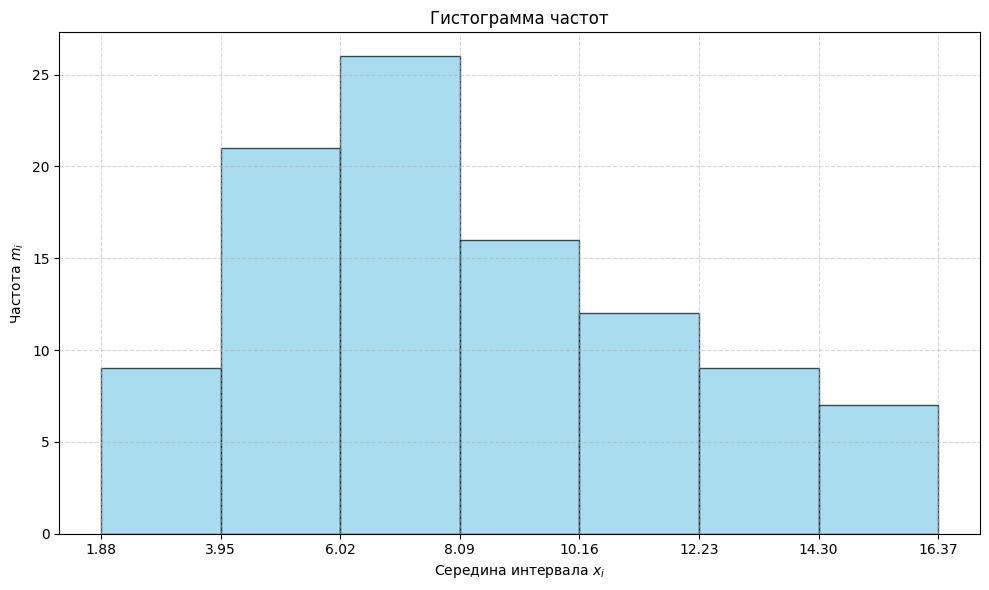
\includegraphics[width=\textwidth]{images/1_histogram.png}
	\end{figure}

	Код:
	\begin{minted}{python}
		plt.figure(figsize=(10, 6))
		plt.hist(X_N, bins=bins, edgecolor='black', alpha=0.7, color='skyblue', density=False)
		plt.title('Гистограмма частот')
		plt.xlabel(r'Середина интервала $x_i$')
		plt.ylabel(r'Частота $m_i$')
		plt.xticks(np.round(bins, 2))
		plt.grid(True, linestyle='--', alpha=0.5)
		plt.tight_layout()
	\end{minted}

	\subsection{Полигон частот}

	Исходя из данных полученных в интервальном ряде (\ref{interval_row}), можно построить полигон частот:
	\begin{figure}[!ht]
		\centering
		\caption{Полигон частот совокупности $X_{18}$ (\ref{X_18})}
		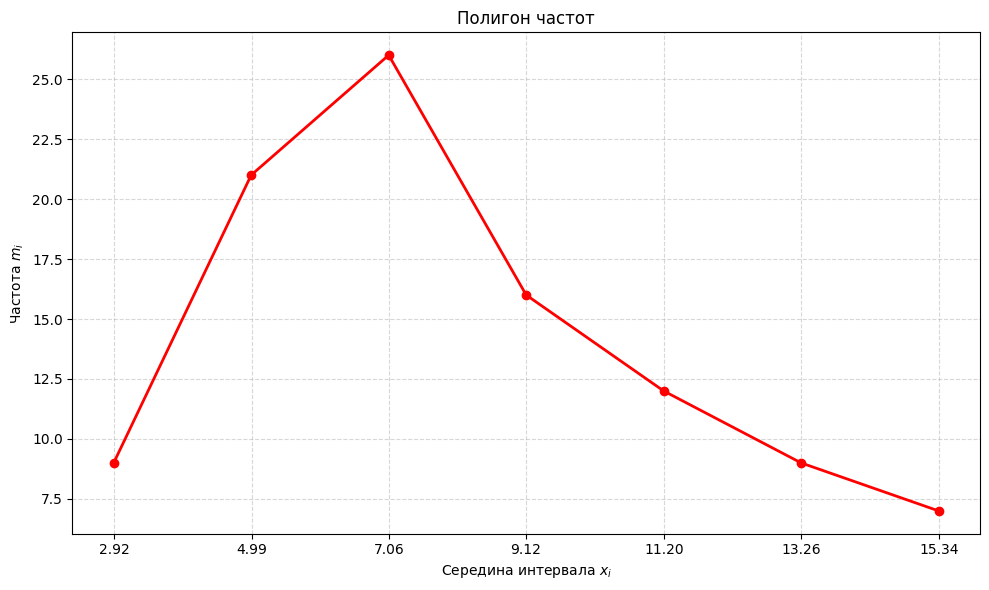
\includegraphics[width=\textwidth]{images/1_polygon.png}
	\end{figure}

	Код:
	\begin{minted}{python}
		bin_centers = (bins[:-1] + bins[1:]) / 2
		plt.figure(figsize=(10, 6))
		plt.plot(bin_centers, counts, marker='o', linestyle='-', color='red', linewidth=2)
		plt.title('Полигон частот')
		plt.xlabel(r'Середина интервала $x_i$')
		plt.ylabel(r'Частота $m_i$')
		plt.xticks(np.round(bin_centers, 2))
		plt.grid(True, linestyle='--', alpha=0.5)
		plt.tight_layout()
	\end{minted}

	\subsection{Эмпирическая функция распределения}

	Эмпирическая функция распределения определяется как:
	\[\displaystyle
	F_X^*(x) = \frac{m_x}{N},
	\]
	где $m_x$ -- число вариант выборки меньше или равно $x$, $N$ -- объём выборки.

	Эмпирическая функция распределения для совокупности $X_{18}$ (\ref{X_18}) выглядит так:
	\begin{figure}[!ht]
		\centering
		\caption{Эмпирическая функция распределения совокупности $X_{18}$ (\ref{X_18})}
		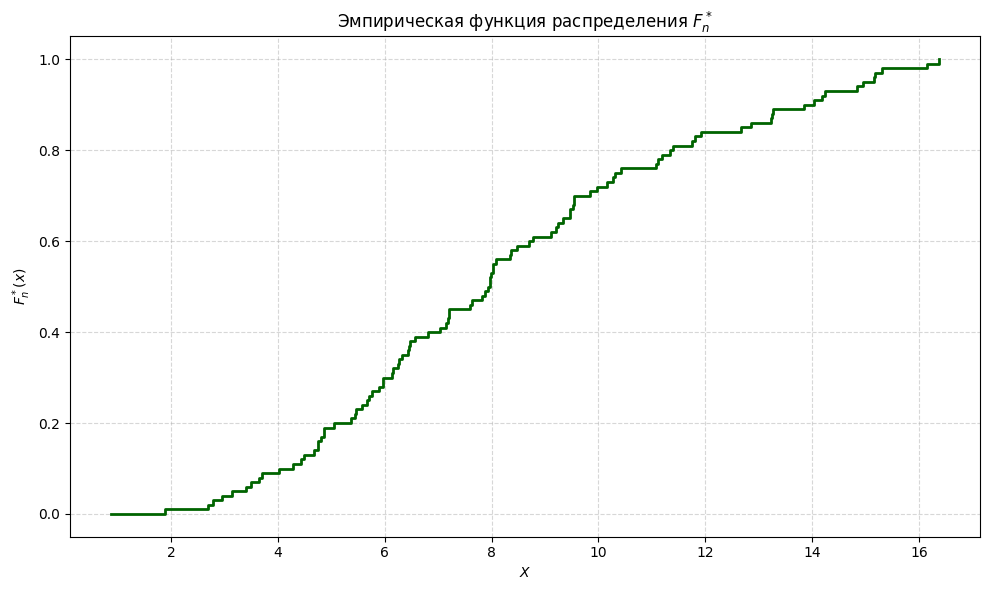
\includegraphics[width=\textwidth]{images/1_ecdf.png}
	\end{figure}

	Код:
	\begin{minted}{python}
		x_sorted = np.sort(X_N)
		y_values = np.arange(1, N + 1) / N
		x_ecdf = np.concatenate(([x_sorted[0] - 1], x_sorted))
		y_ecdf = np.concatenate(([0], y_values))
		plt.figure(figsize=(10, 6))
		plt.step(x_ecdf, y_ecdf, where='post', color='darkgreen', linewidth=2)
		plt.title(r'Эмпирическая функция распределения $F_n^*$')
		plt.xlabel(r'$X$')
		plt.ylabel(r'$F_n^*(x)$')
		plt.ylim(-0.05, 1.05)
		plt.grid(True, linestyle='--', alpha=0.5)
		plt.tight_layout()
	\end{minted}

	\subsection{Выборочные среднее и дисперсия}

	Выборочное среднее вычисляется по формуле:
	\[\displaystyle
	\overline{X}_{18} = \sum_{i = 1}^{N} \frac{x_i}{N} = 8.3139
	\]

	Выборочная дисперсия вычисляется по формуле:
	\[\displaystyle
	\sigma^2_{X_{18}} = \sum_{i = 1}^{N} \frac{(x_i - \overline{X}_{18})^2}{N} = 12.288003789999998
	\]

	Код:
	\begin{minted}{python}
		print(f"Среднее: {np.mean(X_N)}")
		print(f"Дисперсия: {np.var(X_N)}")
	\end{minted}

	\newpage

	\section{задание}
	\subsection{Оценка параметров}

	Оценим параметры равномерного распределения методом максимального правдоподобия: \\
    $\displaystyle
    X \sim U(a, b) \\
    X_1, \ldots, X_n - \text{ выборка из } X \\
    F_X \in \{F(x, a, b) ~|~ a, b \in \mathbb{R}, b \geq a\} \\
    f_X(x) = \frac{I(x \in [a; b])}{(b - a)^n} \\
    L(a, b, X_1, \ldots, X_n) = \prod_{i = 1}^n \frac{I(X_i \in [a; b])}{(b - a)^n} = \frac{1}{(b - a)^n} \prod_{i = 1}^n I(X_i \in [a; b]) \\
    \hat{a}_n = \arg\max_{a \leq b} \frac{1}{(b - a)^n} \prod_{i = 1}^n I(X_i \in [a; b]) = \arg\max_{a \leq X_{\min}} \frac{1}{(b - a)^n} = X_{\min} \\
    \hat{b}_n = \arg\max_{b \geq a} \frac{1}{(b - a)^n} \prod_{i = 1}^n I(X_i \in [a; b]) = \arg\max_{b \geq X_{\max}} \frac{1}{(b - a)^n} = X_{\max} \\
    \text{Оценка параметра } \hat{a}_n = X_{\min} \\
    \text{Оценка параметра } \hat{b}_n = X_{\max} \\
    $

	\subsection{Несмещённость оценки}

	Оценка $\hat{\theta}_n$ является несмещённой, если $E(\hat{\theta}_n) = \theta$

	$\displaystyle
	\text{Математическое ожидание оценки } \hat{a}_n: \\
	P(X_{\min} > x) = P((X_1 > x) \cap \ldots \cap (X_n > x)) = P(X_1 > x) \cdot \ldots \cdot P(X_n > x) \\
	1 - F_{X_{\min}}(x) = 1 - P(X_{\min} \leq x) = (1 - P(X_1 \leq x)) \cdot \ldots \cdot (1 - P(X_n \leq x)) = (1 - F_X(x))^n \\
	F_{X_{\min}}(x) = 1 - (1 - F_X(x))^n \\
	f_{X_{\min}}(x) = \frac{d F_{X_{\min}}}{dx} = n (1 - F_X(x))^{n - 1} f_X(x) = n \left( 1 - \frac{x - a}{b - a} \right)^{n - 1} \frac{1}{b - a} = \frac{n (b - x)^{n - 1}}{(b - a)^n} \\
	E(X_{\min}) = \int_a^b \frac{x n (b - x)^{n - 1}}{(b - a)^n} dx = \frac{na + b}{n + 1} \\
	$

	$\displaystyle
	\text{Математическое ожидание оценки } \hat{b}_n: \\
	F_{X_{\max}}(x) = P(X_{\max} \leq x) = P((X_1 \leq x) \cap \ldots \cap (X_n \leq x)) = P(X_1 \leq x) \cdot \ldots \cdot P(X_n \leq x) = F_X^n(x) \\
	f_{X_{\max}}(x) = \frac{d F_{X_{\max}}}{dx} = n F_X^{n - 1}(x) f_X(x) = n \left( \frac{x - a}{b - a} \right)^{n - 1} \frac{1}{b - a} = \frac{n (x - a)^{n - 1}}{(b - a)^{n}} \\
	E(X_{\max}) = \int_a^b \frac{x n (x - a)^{n - 1}}{(b - a)^{n}} dx = \frac{nb + a}{n + 1} \\
	$
	$
	\left.\begin{array}{c}
		\displaystyle E(\hat{a}_n) = \frac{na + b}{n + 1} \neq a \\
		\displaystyle E(\hat{b}_n) = \frac{nb + a}{n + 1} \neq b
	\end{array}\right\} \Rightarrow
	$
	Оценка смещённая

	\subsection{Состоятельность оценки}

	Оценка $\hat{\theta}_n$ является состоятельной, если $\displaystyle \hat{\theta}_n \xrightarrow{P} \theta \Leftrightarrow \forall \varepsilon > 0 \Rightarrow \lim_{n \rightarrow \infty} P(|\hat{\theta}_n - \theta| < \varepsilon) = 1$

	$\displaystyle
	\text{Предел для оценки } \hat{a}_n: \\
	\lim_{n \rightarrow \infty} P(|\hat{a}_n - a| < \varepsilon) = \lim_{n \rightarrow \infty} P(|X_{\min} - a| < \varepsilon) = \lim_{n \rightarrow \infty} P(X_{\min} - a < \varepsilon) \lim_{n \rightarrow \infty} P(X_{\min} < a + \varepsilon) = \lim_{n \rightarrow \infty} F_{X_{\min}}(a + \varepsilon) = \lim_{n \rightarrow \infty} \left( 1 - \left( \frac{b - a - \varepsilon}{b - a} \right)^n \right) = 1 \\
	$

	$\displaystyle
	\text{Предел для оценки } \hat{b}_n: \\
	\lim_{n \rightarrow \infty} P(|\hat{b}_n - b| < \varepsilon) = \lim_{n \rightarrow \infty} P(|X_{\max} - b| < \varepsilon) = \lim_{n \rightarrow \infty} P(b - X_{\max} < \varepsilon) = \lim_{n \rightarrow \infty} P(X_{\max} > \varepsilon - b) = \lim_{n \rightarrow \infty} (1 - P(X_{\max} \leq b - \varepsilon)) = \lim_{n \rightarrow \infty} (1 - F_{X_{\max}}(b - \varepsilon)) = \lim_{n \rightarrow \infty} \left( 1 - \left( \frac{b - \varepsilon - a}{b - a} \right)^n \right) = 1 \\
	$
	$
	\left.\begin{array}{c}
		\displaystyle \hat{a}_n \xrightarrow{P} a \\
		\displaystyle \hat{b}_n \xrightarrow{P} b
	\end{array}\right\} \Rightarrow
	$
	Оценка состоятельная


\end{document}